\documentclass[review]{elsarticle}

\usepackage{lineno,hyperref}
\modulolinenumbers[5]

\journal{Journal of \LaTeX\ Templates}

%%%%%%%%%%%%%%%%%%%%%%%
%% Elsevier bibliography styles
%%%%%%%%%%%%%%%%%%%%%%%
%% To change the style, put a % in front of the second line of the current style and
%% remove the % from the second line of the style you would like to use.
%%%%%%%%%%%%%%%%%%%%%%%

%% Numbered
%\bibliographystyle{model1-num-names}

%% Numbered without titles
%\bibliographystyle{model1a-num-names}

%% Harvard
%\bibliographystyle{model2-names.bst}\biboptions{authoryear}

%% Vancouver numbered
%\usepackage{numcompress}\bibliographystyle{model3-num-names}

%% Vancouver name/year
%\usepackage{numcompress}\bibliographystyle{model4-names}\biboptions{authoryear}

%% APA style
%\bibliographystyle{model5-names}\biboptions{authoryear}

%% AMA style
%\usepackage{numcompress}\bibliographystyle{model6-num-names}

%% `Elsevier LaTeX' style
\bibliographystyle{elsarticle-num}
%%%%%%%%%%%%%%%%%%%%%%%

\usepackage{amsmath}
\usepackage{amsfonts}
\usepackage{booktabs}

\begin{document}

\begin{frontmatter}

\title{StyleGAN Face Frames}
\tnotetext[mytitlenote]{Fully documented templates are available in the elsarticle package on \href{http://www.ctan.org/tex-archive/macros/latex/contrib/elsarticle}{CTAN}.}

%% Group authors per affiliation:
\author{Roca Agustín, Britos Nicolás Ignacio\fnref{myfootnote}}
\address{C1437FBH Lavarden 315, Ciudad Autónoma de Buenos Aires, Argentina}
\fntext[myfootnote]{Since 1880.}

%% or include affiliations in footnotes:
\author[mymainaddress,mysecondaryaddress]{Instituto Tecnológico de Buenos Aires}
\ead[url]{www.itba.edu.ar}

\author[mysecondaryaddress]{Global Customer Service\corref{mycorrespondingauthor}}
\cortext[mycorrespondingauthor]{Corresponding author}
\ead{support@elsevier.com}

\address[mymainaddress]{1600 John F Kennedy Boulevard, Philadelphia}
\address[mysecondaryaddress]{360 Park Avenue South, New York}

\begin{abstract}
dfjlksjfl;kadjsk;lfjds;alkjfl;dsajf;lkasjd;flkjsaklfjdlaskfjklsadjf



\end{abstract}

\begin{keyword}
StyleGAN
\end{keyword}

\end{frontmatter}

\linenumbers

\section{Introduction}

Introduction 

This paper reports a method to, (1) describe a procedure to capture the shape of a waveform of an ERP component, the P300, using histograms of gradient orientations extracted from images of signal plots, and (2) outline the way in which this procedure can be used to implement an P300-Based BCI Speller application. Its validity is verified by offline processing two datasets, one of data from ALS patients and another one from data of healthy subjects. 

This article unfolds as follows: Section~\ref{Feature} is dedicated to explain the Feature Extraction method based on Histogram of Gradient Orientations of the Signal Plot: Section~\ref{Pipeline} shows the preprocessing pipeline,  Section~\ref{Plot}  describes the image generation of the signal plot, Section~\ref{SIFT}  presents the feature extraction procedure while  Section~\ref{Classification}  introduces the Speller Matrix Letter Identification procedure.  In Section~\ref{Protocol}, the experimental protocol is expounded. Section~\ref{Results} shows the results of applying the proposed technique.  In the final Section~\ref{discussion}  we expose our remarks, conclusions and future work.

\section{Materials and Methods}

fdsafdasfasf

\section{Results} \label{Results}
\label{section:results}

fddafdas
fdsaf

\section{Discussion}
\label{discussion}


\begin{figure}[h!]
\centering
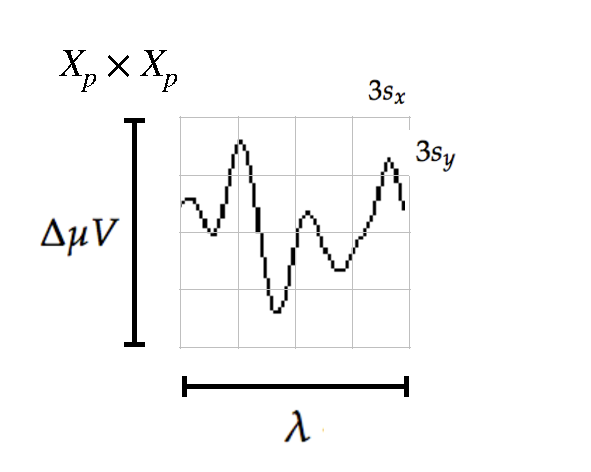
\includegraphics[width=10cm]{patchgeometry.pdf}
\caption{The scale of local patch is selected in order to capture the whole transient event.  The size of the patch is $X_p \times X_p$ pixels. The vertical size consists of $4$ blocks of size $3 s_y$ pixels which is high enough as to contain the signal $\Delta  \mu V $, the peak-to-peak amplitude of the transient event. The horizontal size includes $4$ blocks  of $3 s_x$ and covers the entire duration in seconds of the transient signal event, $ \lambda $.   }
\label{fig:patchgeometry}
\end{figure}

\section{Front matter}

The author names and affiliations could be formatted in two ways:
\begin{enumerate}[(1)]
\item Group the authors per affiliation.
\item Use footnotes to indicate the affiliations.
\end{enumerate}
See the front matter of this document for examples. You are recommended to conform your choice to the journal you are submitting to.

\section{Bibliography styles}

There are various bibliography styles available. You can select the style of your choice in the preamble of this document. These styles are Elsevier styles based on standard styles like Harvard and Vancouver. Please use Bib\TeX\ to generate your bibliography and include DOIs whenever available.

Here are two sample references:

\section*{References}

\bibliography{styleganfaceframe}

\end{document}